\documentclass[12pt,a4paper]{article}
\usepackage[utf8]{vietnam}
\usepackage[margin=10mm]{geometry}
\usepackage{array,color,graphicx,hyperref,tikz}
\usepackage{flowfram}

\pagestyle{empty}
\setlength\parindent{0pt}
\renewcommand{\familydefault}{\sfdefault}

\definecolor{royalblue}{RGB}{65,105,225}
\definecolor{gray}{RGB}{128,128,128}

\newflowframe{.65\textwidth}{.9\textheight} {.35\textwidth}{0pt}
\newdynamicframe{.65\textwidth}{.05\textheight} {.35\textwidth}{.95\textheight}[head]
\newdynamicframe{.3\textwidth}{.15\textheight} {0pt}{.85\textheight}[avt]
\newdynamicframe{.3\textwidth}{.85\textheight} {0pt}{0pt}[left]
\newdynamicframe{.675\textwidth}{.05\textheight} {.325\textwidth}{.9\textheight}[hline]
\newdynamicframe{.05\textwidth}{\textheight} {.3\textwidth}{0pt}[vline]

\begin{dynamiccontents*}{head}
	\begin{flushright}
		\Huge\textbf{C\color{gray}urriculum \color{black}V\color{gray}itae}
	\end{flushright}
\end{dynamiccontents*}

\begin{dynamiccontents*}{avt}
	\begin{center}
		\vspace{-6mm}
		\begin{tikzpicture}[baseline=(avt.center),inner sep=0pt]
			\draw[gray, dashed] (0,0) circle (18.5mm);
			\clip (0,0)  circle (18mm) node (avt) {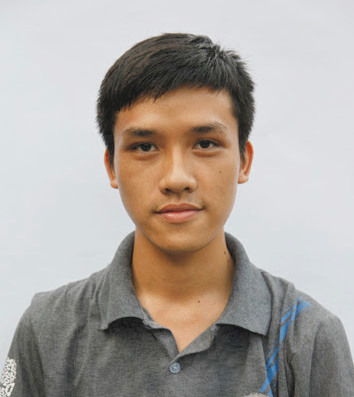
\includegraphics[scale=1.25]{avt.jpg}};
		\end{tikzpicture}
	\end{center}
\end{dynamiccontents*}

\begin{dynamiccontents*}{left}
	\begin{center}
		\textbf{\color{royalblue} NGUYEN PHUOC THINH} \\
		\small STUDENT
	\end{center}
	\begin{flushright}
		\href{mailto:npthinh1996@gmail.com}{npthinh1996@gmail.com} \\
		\url{thinhnguyen.name.vn} \\
		(+84) 989 098 494
		\begin{flushright}
			497 Hoa Hao \\
			Ward 7, District 10 \\
			Ho Chi Minh City
		\end{flushright}
	\end{flushright}
	\begin{flushleft}
		\textbf{About me --}
		\begin{flushleft}
			From a student learn computer engineering, but I have an interest in design and develop website. Present, I want looking for a job about web/python development as a fresher. Please contact me if you interested in my resume.
		\end{flushleft}
	\end{flushleft}
	\begin{flushleft}
		\textbf{Skills --}
		\begin{center}
			\begin{tabular}{m{15mm}  m{33.25mm}}
				HTML & \tikz{\draw[royalblue,line width=5pt] (0,0) -- (33.25mm ,0);} \\
				CSS & \tikz{\draw[royalblue,line width=5pt] (0,0) -- (33.25mm ,0);} \\
				JavaScript & \tikz{\draw[royalblue,line width=5pt] (0,0) -- (15mm ,0);} \\
				PHP & \tikz{\draw[royalblue,line width=5pt] (0,0) -- (25mm ,0);} \\
				Python & \tikz{\draw[royalblue,line width=5pt] (0,0) -- (20mm ,0);} \\
				C++ & \tikz{\draw[royalblue,line width=5pt] (0,0) -- (20mm ,0);} \\
				& \\
				Bootstrap & \tikz{\draw[gray,line width=5pt] (0,0) -- (33.25mm ,0);} \\
				jQuery & \tikz{\draw[gray,line width=5pt] (0,0) -- (10mm ,0);} \\
				WordPress & \tikz{\draw[gray,line width=5pt] (0,0) -- (25mm ,0);} \\
				Laravel & \tikz{\draw[gray,line width=5pt] (0,0) -- (20mm ,0);} \\
				Django & \tikz{\draw[gray,line width=5pt] (0,0) -- (25mm ,0);} \\
				& \\
				Gimp & Photoshop \\
				Git & Heroku \\
				Ubuntu & Docker \\
			\end{tabular}
		\end{center}
	\end{flushleft}
\end{dynamiccontents*}

\begin{dynamiccontents*}{hline}
	\vspace{7mm}
	\hspace{.5mm}
	\tikz{\draw[royalblue,line width=1.5pt,loosely dotted] (0,0) -- (.67\textwidth ,0);}
\end{dynamiccontents*}

\begin{dynamiccontents*}{vline}
	\hspace{3mm}
	\tikz{\draw[royalblue,line width=1.5pt,loosely dotted] (0,0) -- (0,\textheight);}
\end{dynamiccontents*}

\begin{document}
	\textbf{\large\color{royalblue}Personal}
	\begin{itemize}
		\setlength\itemsep{1pt}
		\item Hobbies: Photograph, Music, Travel
		\item Strengths: Friendly, Cautious, Serious
		\item Weaknesses: Quiet, Perfectionist, Foreign Language
	\end{itemize}
	
	\textbf{\large\color{royalblue}Education}
	\begin{center}
		\begin{tabular}{m{20mm}  m{95mm}}
			\color{gray}2014 - 2019 & Bach Khoa University, Ho Chi Minh City \\
			& \textit{\small\color{gray}Computer Science \& Engineering} \\
			\color{gray}2011 - 2014 & Lai Vung 1 High School, Dong Thap Province \\
		\end{tabular}
	\end{center}
		
	\textbf{\large\color{royalblue}Certifications}
	\begin{center}
		\begin{tabular}{m{20mm}  m{95mm}}
			\color{gray}Dec 2018 & TOEIC Listening \& Reading, \href{iigvietnam.com}{IIG Vietnam} \\
			& \textit{\small\small\color{gray}Listening: 235, Reading: 275, Total: 510} \\
			\color{gray}Nov 2018 & \href{http://www.udemy.com/certificate/UC-PRMHJ580}{Python Django Dev To Deployment}, Udemy \\
			& \textit{\small\small\color{gray}License: UC-PRMHJ580} \\
			\color{gray}Sep 2018 & \href{http://www.udemy.com/certificate/UC-53QB9QRM}{Python \& Django Full Stack Web Developer}, Udemy \\
			& \textit{\small\small\color{gray}License UC-53QB9QRM} \\
		\end{tabular}
	\end{center}
	
	\textbf{\large\color{royalblue}Internship}
	\begin{center}
		\begin{tabular}{m{20mm} m{95mm}}
			\color{gray}Jun 2018 & \href{mangoads.vn}{MangoAds}, Ho Chi Minh City \\
			& \textit{\small\small\color{gray}Develop Laravel app and build tool crawl data using Python} \\
		\end{tabular}
	\end{center}
	
	\textbf{\large\color{royalblue}Projects}
	\begin{center}
		\begin{tabular}{m{20mm} m{95mm}}
			\color{gray}Dec 2018 & Using Python to Checking SEO from Another Site \\
			& \textit{\small\small\color{gray}Built by Django and Requests framework} \\
			\color{gray}Jun 2018 & Checking Keywords Rank from Search Enginer \\
			& \textit{\small\small\color{gray}Using Scrapy framework and PHP to build website} \\
			\color{gray}Jan 2017 & Manage Movies Sharing Website \\
			& \textit{\small\small\color{gray}Using WordPress framework, optimize and improve SEO} \\
		\end{tabular}
	\end{center}
	
	\textbf{\large\color{royalblue}Communities}
	\begin{center}
		\begin{tabular}{m{20mm} m{95mm}}
			\color{gray}Jun 2016 & ``Exam Season Support'' Campaign, Ho Chi Minh City \\
			& \textit{\small\small\color{gray}Guiding the travel and supporting the exam procedures} \\
			\color{gray}Jul 2015 & ``Green Summer'' Campaign, Tra Vinh Province \\
			& \textit{\small\small\color{gray}Build the roadways in the countryside and teaching children} \\
		\end{tabular}
	\end{center}
\end{document}
